\documentclass[../main.tex]{subfiles}
\begin{document}
\chapter{Results}
\label{hh:chapter:results}

This chapter presents the results obtained in the CMS \hhbbtt{} analysis using the full Run 2 data set. Two sets of results are produced: inclusive results, considering as signal both ggF and VBF altogether, and VBF-only results, where only the VBF production mode is considered as signal and ggF is fixed to its SM prediction. 

The chapter is structured as follows. Section~\ref{hh:sec:stat} shows an overview of the statistical methodology followed for performing the signal extraction. Section~\ref{hh:sec:systematics} describes the systematic uncertainties considered in the analysis. The final results are shown in Section~\ref{hh:sec:results} and a comparison with the results obtained from other HH analyses is performed in Section~\ref{hh:sec:comparison}.

My main contributions to this chapter are the detailed study of the QCD background estimation, including several tests that try to determine the validity of the estimation method. These validity tests lead to the inclusion of several systematic uncertainties related to the QCD estimation. Additionally, I also studied the uncertainty related to the VBF dipole recoil.

\section{Statistical procedure}
\label{hh:sec:stat}

The statistical methodology used to evaluate the presence or not of signals in data follows the method used in the 2011 combination of the CMS and ATLAS Higgs boson observation results \cite{hh:results:statistical_model}. This procedure, based on the modified frequentist method (often referred to as CL${}_\text{s}$), aims to quantify the compatibility between the observed data and the background plus signal hypothesis or between the data and the background only hypothesis. 

The procedure considers the DNN distributions in the categories (Resolved 1 b-tag, Resolved 2 b-tag, Boosted and 5 VBF subcategories), three channels and three years (from here onwards, event categories) described during the analysis, for both the data, background estimate and signal processes. For each event category, the number of events $n_i$ predicted by the modelling in the bin $i$ of the distribution is defined as
\begin{equation}
n_i(\mu, \boldsymbol{\theta_i})=\mu\cdot s_i (\boldsymbol{\theta_i}) + b_i(\boldsymbol{\theta_i}),
\end{equation}
where $s_i (\boldsymbol{\theta_i})$ and $b_i(\boldsymbol{\theta_i})$ are the modelled signal and background yields in the given bin, $\mu$ is the \textit{signal strength modifier}, defined as the ratio between the observed signal cross section and the one predicted by the SM, and $\boldsymbol{\theta_i}$ are the \textit{nuisance parameters}, which parametrize the different uncertainties. These nuisance parameters are described in Section~\ref{hh:subsec:nuisances}.

\subsection{Observed and expected limits}

In order to estimate the values of the $\mu$ and their associated uncertainties, a binned \textit{likelihood function} is used to quantify the compatibility between the observed data and the prediction for given values of the statistical parameters ($\mu$ and nuisance parameters). This function can be written as the product of the Poisson probabilities to observe $n_i^{obs}$ events in the bin $i$, scaled by the prior nuisance probability distribution (defined in Section~\ref{hh:subsec:nuisances}):
\begin{equation}
L(\mu, \boldsymbol{\theta} | \text{data}) = \prod_i \frac{\left(\mu\cdot s_i (\boldsymbol{\theta_i}) + b_i(\boldsymbol{\theta_i}) \right)^{n_i^\text{obs}}}{n_i^\text{obs}!}e^{(\mu\cdot s_i (\boldsymbol{\theta_i}) + b_i(\boldsymbol{\theta_i}))} \cdot \rho(\boldsymbol{\theta_i}|\boldsymbol{\tilde{\theta_i}})
\end{equation}

To compare the compatibility of the data with  with different signal plus background hypotheses against the background-only hypothesis a \textit{test statistic} $q_\mu$ can be defined as:
\begin{equation}
q_\mu = -2 \ln \frac{L(\mu, \boldsymbol{\hat{\theta}}_\mu | \text{data})}{L(\hat{\mu}, \boldsymbol{\hat{\theta}} | \text{data})},
\end{equation}
where $\hat{\mu}$ and $\boldsymbol{\hat{\theta}}$ are the parameters that maximise $L$, and $\boldsymbol{\hat{\theta}}_\mu$ the set of nuisances that corresponds to the maximum value of $L$ for a given $\mu$ value. Higher values of $q_\mu$ correspond to increasing incompatibility of the data with the signal plus background hypothesis.

The probability density functions $f(q_\mu|\mu,\boldsymbol{\hat{\theta}}_\mu^\text{obs})$ (signal plus background hypothesis) and $f(q_0|0,\boldsymbol{\hat{\theta}}_0^\text{obs})$ (background-only) are obtained by generating pseudo-data, i.e. simulations that follow the same Poisson probability distribution. However, this approach is very CPU consuming, so instead an asymptotic approximation is considered \cite{hh:results:asymptotic}. Instead of using the generated pseudo-data, only the Asimov dataset (where the observations are equal to the predictions and the nuisance parameters are equal to their nominal values) is considered. Thus, the probabilities that the observed value $q_\mu^{n^{\text{obs}}}$ is compatible with the signal plus background ($\equiv$~CL$_{s+b}(\mu)$) or with the background-only ($\equiv$~CL$_{b}$) hypothesis are computed as
\begin{equation}
\begin{matrix}
\text{CL}_{s+b}(\mu) = P(q_\mu \geq q_\mu^{n^{\text{obs}}} | \mu\cdot s + b) = \int_{q_\mu^{n^{\text{obs}}}}^\infty f(q_\mu|\mu, \boldsymbol{\hat{\theta}}_\mu^\text{obs})~\text{d}q_\mu, \\
\text{CL}_{b} = P(q_0 \geq q_0^{n^{\text{obs}}} | b) = \int_{q_0^{n^{\text{obs}}}}^\infty f(q_0|\mu, \boldsymbol{\hat{\theta}}_0^\text{obs})~\text{d}q_0.
\end{matrix}
\end{equation}

Their ratio is known as the $\text{CL}_{s}(\mu)$,
\begin{equation}
\text{CL}_{s}(\mu) = \text{CL}_{s+b}(\mu) / \text{CL}_{b}.
\end{equation}

In the \hhbbtt{} analysis, the confidence level (CL) is taken as the value 1 - $\text{CL}_{s}$. The 95\% CL value ($\text{CL}_{s}(\mu) = 0.05$) is usually chosen as a convention for presenting CMS results.

The observed upper exclusion limit for the signal strength modifier $\mu_{\text{up}}$ is obtained so that $\text{CL}_{s}(\mu_{\text{up}})$ = 0.05. This observed limit can be compared with the expected exclusion limit (i.e. obtained only using the Asimov dataset) and its $\pm1\sigma$ or $\pm2\sigma$ error bands (corresponding to 68\% and 95\% confidence intervals respectively), so the agreement between the observations and the model predictions can be studied. In the asymptotic approach used, the N$\sigma$ error bands $\mu_{\text{up+N}}^\text{exp}$ and the median $\mu_{\text{up}}^\text{exp}$ of the expected limit are obtained using the Asimov dataset and given by \cite{hh:results:asymptotic}
\begin{equation}
\mu_{\text{up+N}}^\text{exp} = \sigma_A\cdot\left(\Phi^{-1}(1 - \text{CL}_s\Phi(N)) + \text{N}  \right),
\end{equation}
where $\sigma^2_A=\mu^2/q_{\mu, A}$ is evaluated by using the Asimov Dataset and $\Phi(x)$ is the cumulative standard Gaussian distribution (zero mean, unit variance).


\subsection{Nuisance parameters}
\label{hh:subsec:nuisances}

Both background and signal event yields are affected by several sources of uncertainties, modelled by introducing nuisance parameters. These nuisance parameters have a probability density function $\rho(\theta|\tilde{\theta})$ associated to some estimate of the nominal value $\tilde{\theta}$ and other parameters regulating its shape. Due to the Bayes' theorem, the probability density can be re-interpreted as a posterior arising from dedicated measurements for the estimations of $\tilde{\theta}$:
\begin{equation}
\rho(\theta|\tilde{\theta}) \sim p(\theta|\tilde{\theta}) \cdot \pi_\theta(\theta),
\end{equation}
where $p(\theta|\tilde{\theta})$ is the probability density function for the auxiliary measurement of $\tilde{\theta}$ and $\pi_\theta(\theta)$ the prior probability distribution.

In the \hhbbtt{} analysis, three types or nuisances are considered. 
\begin{itemize}
\item Normalization uncertainties: some uncertainties only modify the normalization of one or more processes, affecting either all event categories or a limited number of those. Up and down variations of these uncertainties, obtained by adding or subtracting to the bin content the value correspondent to one standard deviation to the central value, vary the number of events of the distribution equally in all bins. The prior probability distributions on these uncertainties involve Gaussian functions. However, for large values of the uncertainties, the normal distribution is not appropriate. Instead, the log-normal distribution is considered:
\begin{equation}
\pi_\theta(\theta) = \frac{1}{\theta}\frac{1}{\sqrt{2\pi}\sigma}\exp\left(-\frac{(\ln\theta)^2}{2\sigma^2}\right),
\end{equation}
where $\sigma$ is the width of the distribution and corresponds to the relative uncertainty on $\theta$, estimated using theoretical calculations or alternative measurements.

\item Shape uncertainties: instead of only modifying the whole integral of the distributions, some uncertainties vary the content of individual bins in an event category distribution. These variations are modelled by recreating the distributions by modifying the quantity affected by the systematic according to the boundaries of its central 68\% confidence interval. Using the three distributions (no variation and up and down variations), the number of events per bin is smoothly interpolated between the boundaries defined by the up and down distributions.

\item Statistical uncertainties: the amount of simulated events that can be produced for a given process per bin and event category is limited. To model the statistical uncertainties, one possibility is to include one separate nuisance per process and bin following a Poisson distribution, the so-called Barlow-Beeston approach \cite{hh:results:barlow_beeston}. However, if enough events are available per bin, the sum of Poisson distributions can be approximated by a Gaussian distribution with reasonable accuracy. In that case, only one nuisance per bin is incorporated in the statistical model.
\end{itemize}


In addition to providing a value for the signal strength modifier, the likelihood maximization provides the best fit values for each nuisance parameter of the statistical model and an estimate of their a-posteriori widths. The nuisance values before and after the fit are referred to as \textit{pre-fit} and \textit{post-fit} values, respectively. %The difference between the central nuisance pre-fit and post-fit values, divided by the width of the pre-fit prior distribution, is called \textit{pull}. A nuisance is \textit{constrained} if its pull is below one.

%To check how important is the effect of a systematic in the fit, its \textit{impact} is computed as the difference between the observed $\mu$ and the obtained when fixing the value of the nuisance to its post-fit value plus and minus its uncertainty, and redoing the fit with the N-1 other nuisances.



\section{Validation tests for the QCD background estimation}
\label{hh:sec:validation_qcd}


In order to evaluate the validity of the followed procedure for the QCD background estimation, several tests were performed. Details and results of these tests are given here.

In the first test, the stability of the estimated QCD normalization has been evaluated by modifying the definition of the C and D regions using four different \deeptau{} working points. These alternative regions are defined as:
\begin{itemize}
\item Events where the \tauh{} passes the VVVLoose working point of the DeepTauVSjet discriminator, but not the VVLoose one.
\item Events where the \tauh{} passes the VVLoose working point of the DeepTauVSjet discriminator, but not the VLoose one.
\item Events where the \tauh{} passes the VLoose working point of the DeepTauVSjet discriminator, but not the Loose one.
\item Events where the \tauh{} passes the Loose working point of the DeepTauVSjet discriminator, but not the Medium one.
\end{itemize}

In these four alternative regions the ratio between the C and D yields is computed and compared with the one obtained with the standard definition of the C and D regions. Results for the C/D yield estimation for the \tauh\tauh{} channel (where the QCD contribution is really important) in 2018 are shown in Fig.~\ref{hh:fig:qcd_test1}. The other channels and years are shown in Appendix~\ref{appendix_b}. A straight line showing a fit to a constant of the C/D yield values for the four alternative working point definitions is also plotted. When a working point leads to a negative yield in either of regions B, C or D, a dashed band is shown and the point is not used to compute the fit nor the average. In general the C/D yield obtained with the standard definition of C and D regions is in agreement within uncertainties with both the result of this constant fit, and with the weighted average of these four alternative C/D yield points. In the few cases where this does not happen, an additional uncertainty is proposed, as defined in Section~\ref{hh:sec:systematics}.

\begin{figure}[h!]
\begin{center}
\subfloat[Boosted]{\includegraphics[width=0.33\textwidth]{Images/qcd_tests/2018/boosted/qcd_inviso__tautau.pdf}}
\subfloat[Resolved 1 b-tag]{\includegraphics[width=0.33\textwidth]{Images/qcd_tests/2018/resolved_1b/qcd_inviso__tautau.pdf}}
\subfloat[Resolved 2 b-tag]{\includegraphics[width=0.33\textwidth]{Images/qcd_tests/2018/resolved_2b/qcd_inviso__tautau.pdf}}\\
\subfloat[VBF subcategory]{\includegraphics[width=0.33\textwidth]{Images/qcd_tests/2018/vbf/hh_vbf_sm_c2v/qcd_inviso__tautau.pdf}}
\subfloat[ggF subcategory]{\includegraphics[width=0.33\textwidth]{Images/qcd_tests/2018/vbf/hh_ggf/qcd_inviso__tautau.pdf}}
\subfloat[$\text{t}\bar{\text{t}}$ subcategory]{\includegraphics[width=0.33\textwidth]{Images/qcd_tests/2018/vbf/tt/qcd_inviso__tautau.pdf}}\\
\subfloat[$\text{t}\bar{\text{t}}$H subcategory]{\includegraphics[width=0.33\textwidth]{Images/qcd_tests/2018/vbf/ttH/qcd_inviso__tautau.pdf}}
\subfloat[DY subcategory]{\includegraphics[width=0.33\textwidth]{Images/qcd_tests//2018/vbf/dy/qcd_inviso__tautau.pdf}}\\
\end{center}
\caption[QCD estimation - First validity test]{C/D yield estimations for the five working points for the \tauh\tauh{} channel in 2018. A dashed band is plotted where the correspondent working point leads to a negative yield for regions B, C and/or D.}
\label{hh:fig:qcd_test1}
\end{figure}

In the second test, the QCD estimation obtained from the ABCD method is compared with a direct data after background subtraction in a sideband region where signal presence is negligible. This sideband region has been defined by inverting the elliptic mass cut from the Resolved 1 b-tag category (defined in Section~\ref{hh:sec:event_categorization}). Fig.~\ref{hh:fig:qcd_test2_dnn} shows the DNN output distribution per channel and year in the sideband region considered. Again, the QCD estimation obtained with the ABCD method has been found to be in good agreement with the direct data-background subtraction in this sideband, validating the QCD estimations obtained with the ABCD method used in the analysis.

\begin{figure}
\centering
\subfloat[$\tau_e\tau_h$, 2016]{\includegraphics[width=0.33\textwidth]{Images/qcd_tests/2016/resolved_1b_inv/DNNoutSM_kl_1__pg_plots__qcd__etau_os_iso__stack}}
\subfloat[$\tau_\mu\tau_h$, 2016]{\includegraphics[width=0.33\textwidth]{Images/qcd_tests/2016/resolved_1b_inv/DNNoutSM_kl_1__pg_plots__qcd__mutau_os_iso__stack}}
\subfloat[$\tau_h\tau_h$, 2016]{\includegraphics[width=0.33\textwidth]{Images/qcd_tests/2016/resolved_1b_inv/DNNoutSM_kl_1__pg_plots__qcd__tautau_os_iso__stack}}\\
\subfloat[$\tau_e\tau_h$, 2017]{\includegraphics[width=0.33\textwidth]{Images/qcd_tests/2017/resolved_1b_inv/DNNoutSM_kl_1__pg_plots__qcd__etau_os_iso__stack}}
\subfloat[$\tau_\mu\tau_h$, 2017]{\includegraphics[width=0.33\textwidth]{Images/qcd_tests/2017/resolved_1b_inv/DNNoutSM_kl_1__pg_plots__qcd__mutau_os_iso__stack}}
\subfloat[$\tau_h\tau_h$, 2017]{\includegraphics[width=0.33\textwidth]{Images/qcd_tests/2017/resolved_1b_inv/DNNoutSM_kl_1__pg_plots__qcd__tautau_os_iso__stack}}\\
\subfloat[$\tau_e\tau_h$, 2018]{\includegraphics[width=0.33\textwidth]{Images/qcd_tests/2018/resolved_1b_inv/DNNoutSM_kl_1__pg_plots__qcd__etau_os_iso__stack}}
\subfloat[$\tau_\mu\tau_h$, 2018]{\includegraphics[width=0.33\textwidth]{Images/qcd_tests/2018/resolved_1b_inv/DNNoutSM_kl_1__pg_plots__qcd__mutau_os_iso__stack}}
\subfloat[$\tau_h\tau_h$, 2018]{\includegraphics[width=0.33\textwidth]{Images/qcd_tests/2018/resolved_1b_inv/DNNoutSM_kl_1__pg_plots__qcd__tautau_os_iso__stack}}
    \caption[QCD estimation - Second validity test]{DNN output distribution per channel for the sideband region defined by inverting the elliptic mass cut in the Resolved 1 b-tag category.  Statistical uncertainties for the data and all background contributions and the normalization systematic uncertainties for the main background processes are included.}
    \label{hh:fig:qcd_test2_dnn}
\end{figure}

Finally, the last validity test consists of obtaining the QCD contribution using the ABCD method in the final analysis categories but redefining the usual regions using an alternative DeepTauVSjet working point that was already introduced in the first test. This way, the new regions A', B', C' and D' use the following selections:
\begin{itemize}
	\item A': Both $\tau$ have opposite charge and the $\tau_h$ passes the VVLoose working point but not the VLoose one.
	\item B': Both $\tau$ have the same charge and the $\tau_h$ passes the VVLoose working point but not the VLoose one.
	\item C': Both $\tau$ have opposite charge and the $\tau_h$ passes the VVVLoose working point but not the VVLoose one.
	\item D': Both $\tau$ have the same charge and the $\tau_h$ passes the VVVLoose working point but not the VVLoose one.
\end{itemize}

This way, we can estimate the QCD contribution in regions close to the analysis signal regions but poorly populated in signal (thanks to considering a very loose working point) and enhanced in QCD contribution. Fig.~\ref{hh:fig:qcd_test3_dnn} shows the DNN output distributions for the \tauh\tauh{} channel in 2018 in this alternative signal region. Agreement within the statistical uncertainties can be seen between the prediction from all background sources, including the QCD estimation obtained with the ABCD method, and the data in this validation region, reassuring the validity of the ABCD method for QCD estimation. In particular, we see a very large QCD contribution in the \tauh\tauh{} channel in the Resolved 1 b-tag category, where also a very good agreement within uncertainties between data and backgrounds can be observed.


\begin{figure}[h!]
\centering
\subfloat[Resolved, 1 b-tag]{\includegraphics[width=0.33\textwidth]{Images/qcd_tests/test3/2018/resolved_1b/DNNoutSM_kl_1__qcd__tautau_os_inviso__vvl_vl__stack__qcd_wp_vvvl_vvl.pdf}}
\subfloat[Resolved, 2 b-tag]{\includegraphics[width=0.33\textwidth]{Images/qcd_tests/test3/2018/resolved_2b/DNNoutSM_kl_1__qcd__tautau_os_inviso__vvl_vl__stack__qcd_wp_vvvl_vvl.pdf}}
\subfloat[Boosted ]{\includegraphics[width=0.33\textwidth]{Images/qcd_tests/test3/2018/boosted/DNNoutSM_kl_1__qcd__tautau_os_inviso__vvl_vl__stack__qcd_wp_vvvl_vvl.pdf}}\\
\subfloat[VBF subcategory]{\includegraphics[width=0.33\textwidth]{Images/qcd_tests/test3/2018/hh_vbf_sm_c2v/DNNoutSM_kl_1_hh_vbf_sm_c2v_merged_mpp__qcd__tautau_os_inviso__vvl_vl__stack__qcd_wp_vvvl_vvl.pdf}}
\subfloat[ggF subcategory]{\includegraphics[width=0.33\textwidth]{Images/qcd_tests/test3/2018/hh_ggf/DNNoutSM_kl_1_hh_ggf_merged_mpp__qcd__tautau_os_inviso__vvl_vl__stack__qcd_wp_vvvl_vvl.pdf}}
\subfloat[$\text{t}\bar{\text{t}}$ subcategory]{\includegraphics[width=0.33\textwidth]{Images/qcd_tests/test3/2018/tt/DNNoutSM_kl_1_tt_merged_mpp__qcd__tautau_os_inviso__vvl_vl__stack__qcd_wp_vvvl_vvl.pdf}}\\
\subfloat[$\text{t}\bar{\text{t}}$H subcategory]{\includegraphics[width=0.33\textwidth]{Images/qcd_tests/test3/2018/tth/DNNoutSM_kl_1_tth_merged_mpp__qcd__tautau_os_inviso__vvl_vl__stack__qcd_wp_vvvl_vvl.pdf}}
\subfloat[DY subcategory ]{\includegraphics[width=0.33\textwidth]{Images/qcd_tests/test3/2018/dy/DNNoutSM_kl_1_dy_merged_mpp__qcd__tautau_os_inviso__vvl_vl__stack__qcd_wp_vvvl_vvl.pdf}}
\caption[QCD estimation - Third validity test]{DNN output distribution for the different analysis categories in the alternative signal region defined by a looser DeepTauVSjet working point for the \tauh\tauh{} channel in 2018. Statistical uncertainties for the data and all background contributions are included.}
\label{hh:fig:qcd_test3_dnn}
\end{figure}




%%%%%%%%%%%%%%%%%%%%%%%%%%%%%%%%%%%%%%%%%%%%%%%%%%%%%%%%%%%%%%%%%%%%%%%%%%%%%%
%%%%%%%%%%%%%%%%%%%%%%%%%%%%%  SYSTEMATICS  %%%%%%%%%%%%%%%%%%%%%%%%%%%%%%%%%%
%%%%%%%%%%%%%%%%%%%%%%%%%%%%%%%%%%%%%%%%%%%%%%%%%%%%%%%%%%%%%%%%%%%%%%%%%%%%%%

\subfile{systematics}

%%%%%%%%%%%%%%%%%%%%%%%%%%%%%%%%%%%%%%%%%%%%%%%%%%%%%%%%%%%%%%%%%%%%%%%%%%%%%%
%%%%%%%%%%%%%%%%%%%%%%%%%%%%%%%%%%%%%%%%%%%%%%%%%%%%%%%%%%%%%%%%%%%%%%%%%%%%%%




\section{Results}
\label{hh:sec:results}

The results shown in this section are obtained by performing a binned maximum likelihood fit of the DNN prediction in eight categories per channel simultaneously for all three years, resulting in a total of 72 input distributions. The three types of nuisance parameters introduced in Section~\ref{hh:subsec:nuisances} are considered, being the normalization and systematic uncertainties further described in Section~\ref{hh:sec:systematics}. 

The DNN output distributions in 2018 for the $\tau_h\tau_h$ channel in the eight analysis categories is shown in Fig.~\ref{hh:fig:dnn_tautau}. The binning schemes used in the DNN distributions are chosen to minimise the expected upper limit, while keeping as low as possible the number of bins per distribution and ensuring the stability of the fit. Each bin is required to contain at least one t$\bar{\text{t}}$ and one Z$/\gamma^*$~+~jets event and to have a weighted background yield larger than 0.03. The uncertainty bands shown in the distributions are the post-fit ones. The other channels and years can be found in Ref.~\cite{hh:results:public_hhbbtt}.

%\begin{figure}
%\begin{center}
%\includegraphics[width=\textwidth]{Images/DNNplots_muTau_2018}
%\end{center}
%\caption{DNN prediction distributions in the \taumu\tauh{} channel in 2018 for the eight analysis categories. The shaded band in the plots represents the statistical plus systematic uncertainty. \textcolor{red}{Fuente de las figuras suplementarias?}}
%\label{hh:fig:dnn_mutau}
%\end{figure}
%
%\begin{figure}
%\begin{center}
%\includegraphics[width=\textwidth]{Images/DNNplots_eTau_2018}
%\end{center}
%\caption{DNN prediction distributions in the \taue\tauh{} channel in 2018 for the eight analysis categories. The shaded band in the plots represents the statistical plus systematic uncertainty. \textcolor{red}{Fuente de las figuras suplementarias?}}
%\label{hh:fig:dnn_etau}
%\end{figure}


\begin{figure}
\begin{center}
\includegraphics[width=\textwidth]{Images/DNNplots_tauTau_2018}
\end{center}
\caption[DNN output distributions in the \tauh\tauh{} channel in 2018]{DNN output distributions in the \tauh\tauh{} channel in 2018 for the eight analysis categories. The shaded band in the plots represents the statistical plus systematic uncertainty. Extracted from \cite{hh:results:public_hhbbtt}.}
\label{hh:fig:dnn_tautau}
\end{figure}



The expected and observed limits for the ggF + VBF HH production cross section at the SM and those for the VBF only HH production cross section are listed in Tables~\ref{hh:tab:limit_r} and \ref{hh:tab:limit_rvbf}, respectively. A visual representation of these limits is provided in Fig.~\ref{hh:fig:limits_r}.

\begin{table}[h!]
\begin{center}
\begin{tabular}{l | r | r}
& 
$
\begin{matrix}
\text{Obs. (Exp.) limit on } \\ \sigma_{\text{ggF+VBF}}(\text{pp}\to\text{HH})/ \sigma_{\text{ggF+VBF}}^{\text{theory}} 
\end{matrix}
$
& 
$
\begin{matrix}
\text{Obs. (Exp.) limit on } \\ \sigma_{\text{ggF+VBF}}(\text{pp}\to\text{HH}) \text{~[fb]}
\end{matrix}
$ \\ \hline
2016 &     8.9 (10.6) & 272 (324) \\
2017 &     9.5 (11.7) & 291 (356) \\
2018 &     5.5 (8.2)  & 169 (249) \\
Combined & 3.3 (5.2)  & 102 (159)
\end{tabular}
\end{center}
\caption[Upper limits on the HH inclusive production cross section]{Expected and observed upper limits on the ratio of the experimentally expected at 95\% CL for the SM point, where $\sigma_{\text{ggF+VBF}}^{\text{theory}}=32.776$~fb is the sum of the ggF and VBF HH production modes cross sections.}
\label{hh:tab:limit_r}
\end{table}


\begin{table}[h!]
\begin{center}
\begin{tabular}{l | r | r}
& 
$
\begin{matrix}
\text{Obs. (Exp.) limit on } \\ \sigma_{\text{VBF}}(\text{pp}\to\text{qqHH})/ \sigma_{\text{VBF}}^{\text{theory}} 
\end{matrix}
$
& 
$
\begin{matrix}
\text{Obs. (Exp.) limit on } \\ \sigma_{\text{VBF}}(\text{pp}\to\text{qqHH}) \text{~[fb]}
\end{matrix}
$ \\ \hline
2016 &     283 (357) & 487 (616) \\
2017 &     280 (392) & 485 (676) \\
2018 &     241 (226) & 414 (391) \\
Combined & 124 (154) & 212 (266)
\end{tabular}
\end{center}
\caption[Upper limits on the HH VBF-only production cross section]{Expected and observed upper limits on the ratio of the experimentally expected  at 95\% CL for the SM point, where $\sigma_{\text{VBF}}^{\text{theory}}=1.726$~fb is the VBF HH production mode cross section.}
\label{hh:tab:limit_rvbf}
\end{table}


\begin{figure}[h!]
\begin{center}
\subfloat{\includegraphics[width=0.5\textwidth]{Images/Figure_007-a}}
\subfloat{\includegraphics[width=0.5\textwidth]{Images/Figure_007-b}}
\end{center}
\caption[Upper limits on the inclusive and VBF-only production cross sections]{Expected and observed upper limits on the ratio of experimentally expected (left) ggF + VBF ($\sigma_{\text{ggF+VBF}}$) and (right) VBF only ($\sigma_{\text{VBF}}$) HH production cross section and the expectation from the SM ($\sigma_\text{theory}$) at 95\%, split by the different years and combined for the full Run 2 dataset. Extracted from \cite{hh:analysis:run2}.}
\label{hh:fig:limits_r}
\end{figure}

In order to study the Higgs couplings involved, the upper limits on the HH production cross section can also be computed for fixed values of the parameters. Fig.~\ref{hh:fig:scans_r} shows the scans of the expected and observed upper limits on the HH production cross sections as functions of $\kappa_\lambda$ (ggF + VBF) and \kvv{} (VBF only). With 95\% CL, $\kappa_\lambda$ gets constrained between $ -1.7 <\kappa_\lambda < 8.7$ (observed) and $-2.9 < \kappa_\lambda < 9.8$ (expected) and \kvv{} between $-0.4 <$~\kvv{}~$< 2.6$ (observed) and $-0.6<$~\kvv{}~$<  2.8$ (expected). In both cases, the other couplings are set to 1 (i.e. SM value).

\begin{figure}[h!]
\begin{center}
\subfloat{\includegraphics[width=0.5\textwidth]{Images/Figure_008-a}}
\subfloat{\includegraphics[width=0.5\textwidth]{Images/Figure_008-b}}
\end{center}
\caption[Constraints for $\kappa_\lambda$]{Expected and observed upper limits on the experimentally expected (left) ggF + VBF ($\sigma_{\text{ggF+VBF}}$) HH production cross section as functions of $\kappa_\lambda$ and (right) VBF only ($\sigma_{\text{VBF}}$) HH production cross section as functions of \kvv. In both cases, all the other couplings are set to their SM expectations. The red solid lines show the theoretical prediction for the HH production cross sections and its uncertainty (red shaded bands). Extracted from \cite{hh:analysis:run2}.}
\label{hh:fig:scans_r}
\end{figure}

%Fig.~\ref{hh:fig:limits_r} shows the two-dimensional scans of the expected and observed upper limits on the HH production cross sections as functions of $\kappa_\lambda$ and $\kappa_t$ (ggF + VBF) and \kvv{} and $\kappa_V$ (VBF only). A point in a two-dimensional parameter space is excluded when the upper limit on HH production cross section at 95\% CL is measured to be below the theoretical cross section, evaluated at the corresponding parameter values. In both diagrams, the SM point is included inside the constrained area.
%
%
%\begin{figure}[h!]
%\begin{center}
%\subfloat{\includegraphics[width=0.5\textwidth]{Images/Figure_009-a}}
%\subfloat{\includegraphics[width=0.5\textwidth]{Images/Figure_009-b}}
%\end{center}
%\caption{Two-dimensional exclusion regions for the full Run-2 combination as a function (left) of $\kappa_\lambda$ and $\kappa_t$ with \kvv and $\kappa_V$ set to unity and (right) of \kvv{} and $\kappa_V$, with both $\kappa_\lambda$ and $\kappa_t$ fixed to unity. Expected uncertainties on exclusion boundaries are inferred from uncertainty bands of the limit calculation, and are denoted by dark and light-grey areas. The blue area marks parameter combinations observed to be excluded. Theoretical cross section values are illustrated by thin, labeled contour lines with the SM prediction (i.e. all parameters set to unity) denoted by a red diamond. Extracted from \cite{hh:analysis:run2}.}
%\label{hh:fig:limits_r_2d}
%\end{figure}

For both the ggF and VBF results reported, the largest sensitivity comes from the \tauh\tauh{} channel, followed by the \taumu\tauh{} and the \taue\tauh{} channels. The Resolved, 2 b-tag category provides the largest sensitivity when constraining the $\kappa_\lambda$ value, while the VBF subcategory is the most dominant in the \kvv{} measurement.

%The impacts of the 25 highest ranked uncertainties in the ggF+VBF signal strength are shown in Fig.~\ref{hh:fig:pulls_impacts} for the full Run 2 fit. Most of these uncertainties are statistical-related, arising from the application of the Barlow-Beeston method. The highest impact comes from the uncertainty in the cross section of the HH production via ggF. This impact is also very one-sided, as is the uncertainty range $\left({}^{+6\%}_{-23\%}\right)$. Two uncertainties related to the QCD background estimation are present, both related to the Resolved, 2 b-tag category and the \tauh\tauh channel in 2016. The impact of the normalization uncertainty (represented as CMS\_bbtt\_res2b\_tauTau\_2016\_QCDratio) come from the actual value of the uncertainty, which was among the highest (118.5\%). Regarding the shape uncertainty, Fig.~\ref{hh:fig:dnn_res2b_2016_tautau} shows the distribution of the DNN discriminant in this channel, category, and year in two regions used for QCD estimation: B (same sign, isolated), whose shape is taken as up template for the shape uncertainty, and C (opposite sign, non-isolated), whose shape is taken as down template. Region B has much smaller statistics than region C, and data fluctuations in the last bins (which are the most sensitive) increase the impact of this uncertainty. As this category, channel, and year are among the most sensitive for the inclusive ggF+VBF analysis, the two uncertainties are ranked as two of the ones with the most impact.

%\begin{figure}[h!]
%\begin{center}
%\includegraphics[page=1,width=\textwidth]{Images/pulls_impacts_unblinded}
%\end{center}
%\caption[Pulls and impacts]{Pulls and impacts of the 25 uncertainties with the highest ranking on the measured ggF+VBF signal strength for the full Run 2 fit.}
%\label{hh:fig:pulls_impacts}
%\end{figure}
%
%\begin{figure}[h!]
%\begin{center}
%\subfloat{\includegraphics[width=0.49\textwidth]{Images/dnn_tautau_2016_res2b_ssiso}}
%\subfloat{\includegraphics[width=0.49\textwidth]{Images/dnn_tautau_2016_res2b_osinviso}}
%\end{center}
%\caption[DNN discriminant in region B, \tauh\tauh{} channel, and Resolved 2 b-tag category in 2016]{DNN discriminant in regions B (same sign, isolated) (left) and C (opposite sign, non-isolated) for the \tauh\tauh{} channel, Resolved 2 b-tag category in 2016.}
%\label{hh:fig:dnn_res2b_2016_tautau}
%\end{figure}


\section{Comparison with other HH analyses}
\label{hh:sec:comparison}

\begin{figure}[h!]
\begin{center}
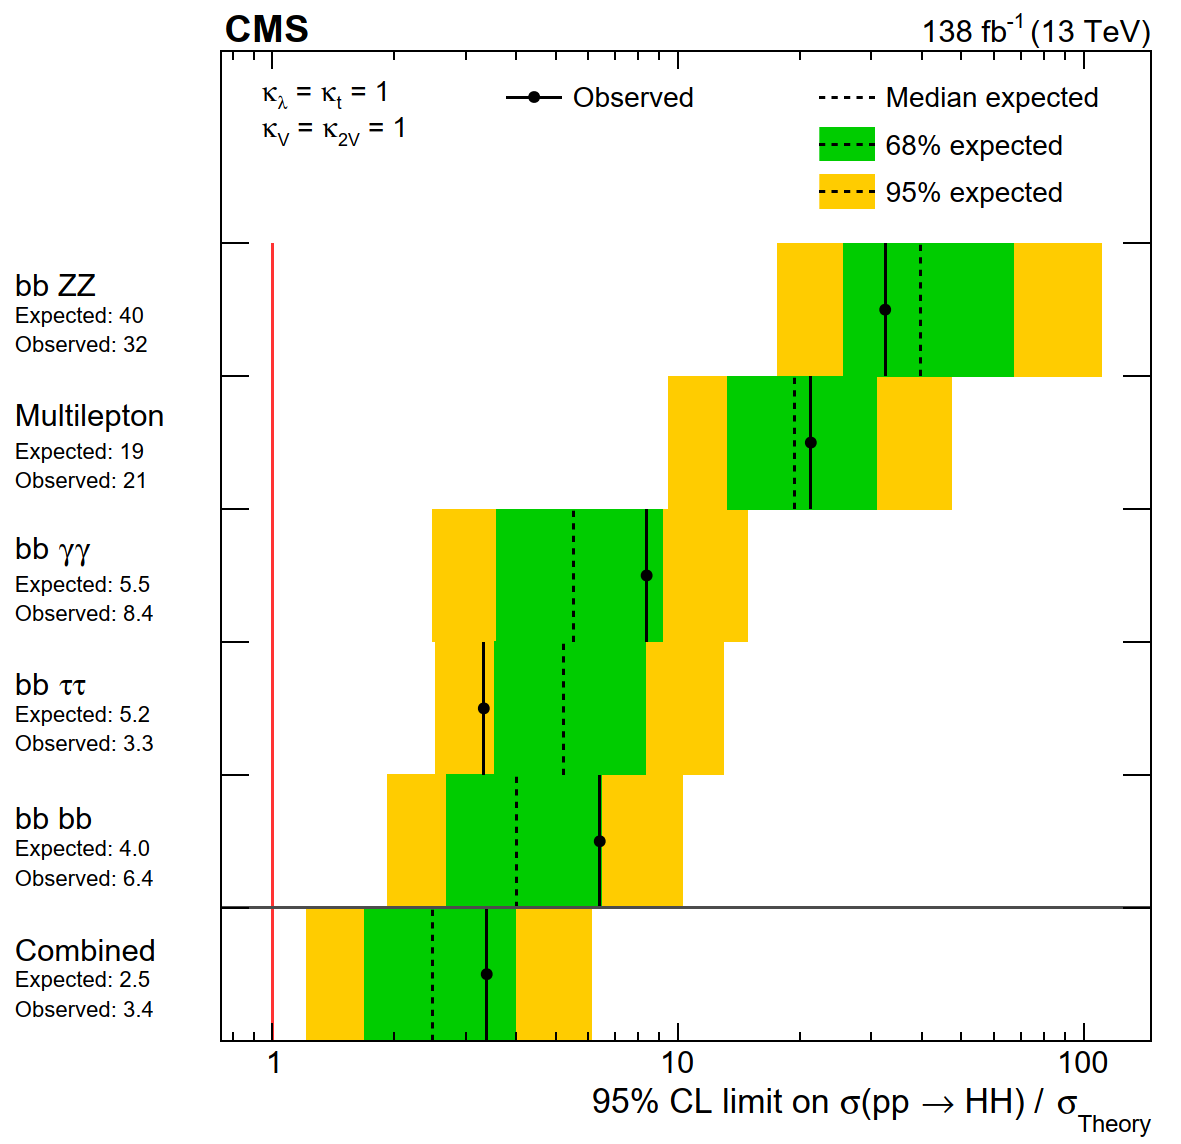
\includegraphics[width=0.7\textwidth]{Images/CMS-HIG-22-001_Figure_005-a}
\end{center}
\caption[CMS HH production cross section results]{Expected and observed limits on the ratio of experimentally estimated production cross section and the expectation from the SM $\sigma_{\text{Theory}}$ in searches using different final states and their combination. The search modes are ordered, from upper to lower, by their expected sensitivities from the least to the most sensitive. The overall combination of all searches is shown by the lowest entry. Extracted from \cite{hh:analysis:nature}.}
\label{hh:fig:lim_comb}
\end{figure}

In this section a comparison between the results shown above and the ones provided by other analyses is performed.

First, within CMS the most direct comparison is with the \hhbbtt{} analysis using 2016 data published in 2018 \cite{hh:analysis:2016}. In this analysis, the signal extraction was performed by fitting the $m_{T2}$ distribution \cite{hh:analysis:mt2} and a BDT was used in order to identify and reject the t$\bar{\text{t}}$ background. The observed (expected) limit on the measured HH production cross section at the SM point times the bb$\tau\tau$ branching fraction was found to be 75.4(61.0)~fb, correspondent to 31.5(25.5) times the cross section predicted by the SM. These numbers can be directly compared with the upper limits obtained in latest analysis using only 2016 data, shown in Tab.~\ref{hh:tab:limit_r} (observed (expected) limit of 8.9(11.0) times the SM prediction). Therefore, in the full Run-2 analysis we can see an improvement of $\sim$58\% in the expected limit and $\sim$70\% in the observed limit. Regarding the $\kappa_\lambda$ measurement, the 2016 analysis obtained observed (expected) constraints of $-18(-14) < k_\lambda < 26(22)$, a much wider range than the one obtained in the full Run-2 analysis. These new results benefit from the improved trigger strategy and the adoption of new techniques not only at analysis level, with the new neural network approaches used for categorization and signal extraction, but in the identification and reconstruction algorithms developed within the CMS Collaboration.

Considering the full Run-2 dataset, the ATLAS Collaboration also performed a \hhbbtt{} search \cite{hh:analysis:atlas, hh:analysis:atlas_comb}. Similarly to the CMS analysis, the signal extraction is performed by fitting the output score of a multivariate approach. Assuming a $\sigma_{\text{ggF+VBF}}^{\text{theory}}=32.7$~fb, the observed (expected) upper limit on the HH production cross section obtained was 4.7(3.9) times $\sigma_{\text{ggF+VBF}}^{\text{theory}}$. The value of $\kappa_\lambda$ is constrained between $-2.5 < \kappa_\lambda < 9.3$ (observed) and $-1.9 < \kappa_\lambda < 9.1$ (expected). These results are a bit more stringent than the CMS ones.

With respect to the VBF HH production, ATLAS did not perform a dedicated analysis for this production mode, although some results on the production cross section and the \kvv{} constraints were provided in the combination of ATLAS HH results \cite{hh:analysis:atlas_comb}. The observed (expected) upper limit on the VBF HH production cross section was found to be 433(366)~fb, while \kvv{} is constrained between $-0.5<~$\kvv{}$~<2.7$ (observed and expected). The value of the upper limit is much larger with respect to the one obtained in the CMS analysis. In fact, the CMS \hhbbtt{} analysis provides a lower limit than every decay channels studied in ATLAS. Regarding \kvv{}, its constraints are quite similar to the ones obtained in the CMS analysis.

Regarding other CMS HH searches with Run-2 data, a combination of the CMS HH results was published to celebrate the tenth anniversary of the Higgs boson discovery \cite{hh:analysis:nature}. This combination includes five final states, and the bb$\tau\tau$ analysis ranks among the first three with the highest sensitivity (see Fig.~\ref{hh:fig:lim_comb}). 

\section{Future prospects}

Given the importance of the Higgs pair production in the SM and to test BSM theories, searches for this production will be conducted with data taken during Run 3 (2022-2025) and HL-LHC (2029-).

During Run 3, CMS will collect around 220~fb$^{-1}$. With this increase in statistics, the expected upper limit on the inclusive HH production cross section obtained by the \hhbbtt{} analysis could be lowered to $\sim3.2$ times the SM prediction. However, new techniques are being studied already for their inclusion in a future Run 3 analysis, such as the identification of $\tau_h$ and jets using particle clouds \cite{hh:results:particlenet}. Additionally, a new trigger strategy has been studied for the \tauh\tauh{} channel in Run 3, providing a sensitivity increase of up to 10\%. This trigger strategy is described in Chapter~\ref{hh:chapter:trigger}.

The prospects for the study of the Higgs boson pair production after HL-LHC have been conducted by both CMS and ATLAS experiments \cite{hh:analysis:nature, hh:results:future, hh:analysis:hh_hllhc}. These projection studies assume a total integrated luminosity of 3000~fb${}^{-1}$, and take into account the upcoming detector upgrades and state-of-the-art analysis techniques. 

The CMS \hhbbtt{} projection \cite{hh:analysis:hh_hllhc} follows an analysis strategy similar to the Run 2 analysis presented in this thesis: two b-tagged jets and two leptons are selected, although only the fully-hadronic (\tauh\tauh{}) and semi-leptonic (\taumu\tauh{}, \taue\tauh{}) decay channels are considered. Signal extraction is performed with a neural network that follows the same approach as the one described in this thesis. By fitting the expected DNN output distributions in the three final states considered, the expected upper limit on the measured HH production cross section at the SM point times the bb$\tau\tau$ branching fraction was found to be 1.4 times the SM prediction. Fig.~\ref{hh:fig:lim_future} shows a comparison between the upper limits obtained with early Run 2 data, full Run 2, and the projection for HL-LHC for the bbbb, bb$\tau\tau$, and bb$\gamma\gamma$ CMS analyses, and the results for the three decay channels combined. Something to be noted is that, as the combined limit after HL-LHC is expected to be below unity, the sensitivity could be sufficient to establish the existence of the SM HH production. In fact, when combining the results of CMS and ATLAS after HL-LHC, a significance of 4 standard deviations could be achieved, providing an evidence of the existence of SM HH production \cite{hh:results:future}.

\begin{figure}[h!]
\begin{center}
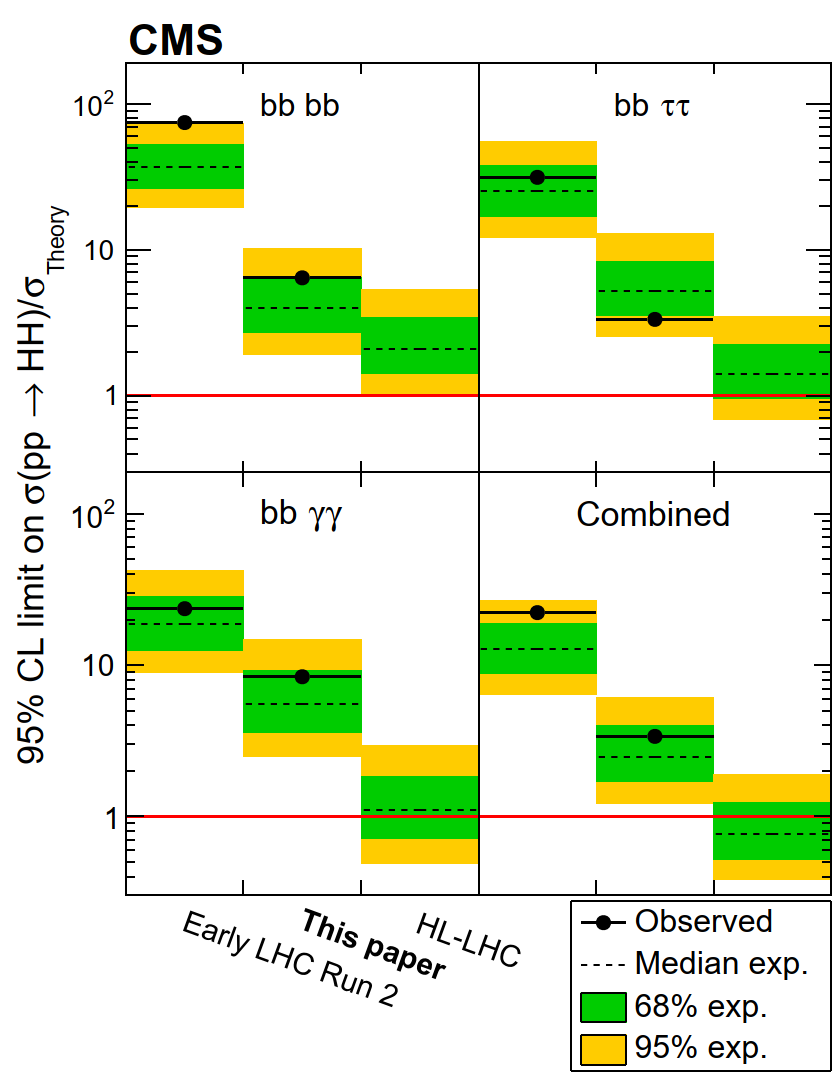
\includegraphics[width=0.6\textwidth]{Images/CMS-HIG-22-001_Figure_005-b}
\end{center}
\caption[CMS HH production cross section for different datasets.]{Expected and observed limits on HH production in different datasets: early LHC Run 2 data (35.9~fb${}^{-1}$), present results using full LHC Run 2 data (138~fb${}^{-1}$), and projections for HL-LHC (3000~fb${}^-1$). Extracted from \cite{hh:analysis:nature}.}
\label{hh:fig:lim_future}
\end{figure}

Even if these projections already assume an improvement on the theoretical predictions (scaling down the theoretical uncertainties) and an upgraded CMS detector (scaling down the experimental uncertainties), there is still room for improving these results. For instance, the \tauh{} and b jet identification algorithms used in the Run 2 analysis (DeepTau and HH-btag, respectively) are not considered in these projections. Moreover, all techniques that are being studied for Run 3 could boost the sensitivity in this future HL-LHC analyses.


\section{Summary}

This chapter includes the results for the search for Higgs boson pair production using Run 2 proton-proton collision data at 13~TeV, where one Higgs boson decays into two $\tau$ leptons and the other into two b quarks. Two sets of results have been shown: inclusive results, where both ggF and VBF production modes are considered as signal, and VBF-only results, where only the VBF production mode is considered as signal and the ggF signal strength is fixed to its SM prediction.

The statistical procedure followed to obtain these results has been described. It is based on a binned maximum likelihood fit for the DNN discriminator described in Chapter~\ref{hh:chapter:analysis}. A complete description of the systematic uncertainties affecting the analysis has been included, coming from experimental and theoretical sources. Among the first ones, several uncertainties affecting the QCD contribution are included, coming from a set of validity tests I performed to study the QCD background estimation method. Additionally, among the theoretical uncertainties I have studied the uncertainty coming from the modelling of the dipole recoil in the HH VBF samples.

The observed (expected) upper limit with a 95\% CL on inclusive HH production cross section corresponds to 3.3 (5.2) times the theoretical cross section predicted by the SM. For the VBF-only production, the limit is set at 124 (154) times the SM prediction. Additionally, 95\% constraints have been established on the Higgs self-coupling ($\kappa_\lambda$) and its coupling to the vector bosons (\kvv), as deviations of these couplings could be produced by BSM effects. For $\kappa_\lambda$, the observed (expected) constraint has been set to $-1.7 < \kappa_\lambda < 8.7$ ($-2.9 < \kappa_\lambda < 9.8$). For \kvv{}, the obtained constraint was $-0.4 < \kappa_{2V} < 2.6$ ($-0.6 < \kappa_{2V} < 2.8$).

Regarding the inclusive results, the full Run-2 analysis shows a large improvement with respect to the previously published CMS \hhbbtt{} results (using 2016 data). This improvement comes not only from the larger statistics but from the inclusion of a new trigger strategy and the adoption of new techniques at analysis level. Additionally, new particle identification and reconstruction algorithms developed within the CMS Collaboration have been considered. With respect to the ATLAS Collaboration \hhbbtt{} search, the results are very similar. Within the CMS Collaboration, the \hhbbtt{} result ranks among the most sensitive HH decay channels under study. Regarding the VBF-only results, the CMS \hhbbtt{} analysis provides a better sensitivity than the ATLAS analysis.

Looking into the future, the CMS and ATLAS Collaborations have conducted projections for the HH analyses after HL-LHC. For the CMS \hhbbtt{} analysis, an expected upper limit on the HH production cross section times the branching fraction of 1.4 times the SM prediction is obtained. A combination of the CMS and ATLAS results after HL-LHC is expected to provide the first evidence of HH production, with a significance of 4 standard deviations. However, there is room for improvement thanks to, among others, the inclusion of new particle identification techniques or a new trigger strategy.



\end{document}

